% ======================================================================
%  A First Defense: Weight-Space Detection of the Pruning Backdoor
%  Requires: \usepackage{booktabs} \usepackage{graphicx}
%  Figures: defense_fig_gemma2.png , defense_fig_qwen.png
%  NOTE: the \clearpage below flushes all floats (tables/figures) from the
%  preceding calibration section, so this section's tables do not interleave
%  with it. Keep it, or replace with \FloatBarrier (needs \usepackage{placeins}).
% ======================================================================
\clearpage
\subsection{A First Defense: Weight-Space Detection}
\label{sec:defense}

\paragraph{Motivation.}
Our stealth evaluation so far is behavioral only (attack-success rate plus benign refusal rate). A
natural question is whether the edit is visible in the \emph{weights}. We therefore design
weight-space detectors, ask whether they catch the attack, and---because a defense is only meaningful
against an adaptive adversary---test them against a trivial camouflage and against honest fine-tunes.
This turns the contribution from ``here is an attack'' into ``here is an attack, a first detector, and
its limits.''

\paragraph{Detectors.}
We consider three, in increasing order of deployability.
\emph{Detector~A (base-relative edit norm)} needs the public base model: it reports
$\lVert W_{\text{att}}-W_{\text{base}}\rVert / \lVert W_{\text{base}}\rVert$ per (layer, module).
\emph{Detector~B (base-free tail anomaly)} needs only the suspect checkpoint and any calibration set:
per \texttt{down\_proj} layer it computes
$\text{tail\_ratio} = \operatorname{mean}|W|_{\text{bottom-}12\%\ \text{importance}} / \operatorname{mean}|W|_{\text{all}}$,
exploiting that the repair deliberately places \emph{large} weights on \emph{low}-importance columns.
Detector~B in this raw form has two failure modes, which motivate the localized variant below.
First, it is \emph{not threshold-separable}: it flags the strongly-edited layers ($8$--$14$,
tail-ratio $1.12$--$1.73\times$ base) but the weakly-edited layers ($18$--$22$, $\approx 1.03\times$)
fall inside the natural layer-to-layer variation of the model---a clean layer's tail-ratio can exceed
a weakly-edited one---so no single absolute threshold cleanly separates edited from clean (AUC
$0.911$, not a usable operating point). Second, it has a \emph{high false-positive rate}: ordinary
supervised fine-tuning broadly increases weight magnitude on low-importance columns, which mimics
exactly the statistic the repair produces; an honest summarization fine-tune therefore trips an
absolute tail-ratio threshold on $25/26$ layers---worse than the attack itself. The root problem is
that B reads an \emph{absolute magnitude}, whereas the attack's true signature is \emph{where} the
anomaly sits, not how large it is.

\emph{Detector~B2 (localized, base-relative)}---the deployable version---fixes both by scoring the
\emph{localization} of the anomaly instead of its magnitude. It takes the per-layer anomaly
$\delta_i = \text{tail\_ratio}_{\text{suspect},i} - \text{tail\_ratio}_{\text{base},i}$, converts it to a
robust within-model outlier score $z_i = (\delta_i - \operatorname{median})/(1.4826\cdot\text{MAD})$,
and \textbf{flags the model if $\geq 2$ layers have $z_i > 4$}. The rationale is that the attack is
\emph{sparse} (spikes on the edited layers, which become high-$z$ outliers) whereas honest fine-tunes
are \emph{diffuse} (a uniform shift that raises the median and MAD together and is therefore absorbed,
yielding no outliers). This directly resolves B's false positives: the summarization fine-tune that
trips absolute-B on $25/26$ layers produces $0$ localized flags.

\paragraph{What we measure.}
(i) Whether each detector separates the attacked model from clean controls; (ii) robustness to an
adaptive attacker who ships the edit as a ``fine-tune'' by adding isotropic Gaussian noise of relative
magnitude $\sigma$ to \emph{all} weight matrices (Table~\ref{tab:defense-noise}), while we track that
the attack still works (unpruned stays benign, pruned still fires); and (iii) for B2, the
true-/false-positive behavior against panels of honest public fine-tunes across two model families
(Table~\ref{tab:defense-b2}), together with the per-layer localization signature
(Figures~\ref{fig:defense-gemma2},~\ref{fig:defense-qwen}).

% ---------- Table 1: adaptive noise camouflage ----------
\begin{table}[t]
\centering
\small
\begin{tabular}{l cccc}
\toprule
Noise $\sigma$ & Detector A sep.\ & Detector B & Unpruned & Pruned \\
(rel.) & (edited/clean) & AUC & ASR & (Wanda-30) ASR \\
\midrule
$0$ (naive) & $1.4\!\times\!10^{10}$ & $0.911$ & $6.5\%$ & $75.5\%$ \\
$0.001$     & $17\times$             & $0.911$ & $6.5\%$ & $73.5\%$ \\
$0.01$      & $1.7\times$ (dead)     & $0.911$ & $6.0\%$ & $73.5\%$ \\
\bottomrule
\end{tabular}
\caption{Adaptive ``fine-tune'' camouflage (Gemma2-2B). Isotropic noise on all weight matrices
collapses Detector~A (edited/clean separation falls from $10^{10}$ to overlap) at essentially no cost
to the attack (pruned ASR stays $\approx 74\%$, unpruned stays benign). Detector~B, which reads a
local magnitude anomaly rather than a base difference, is noise-invariant.}
\label{tab:defense-noise}
\end{table}

% ---------- Table 2: B2 across architectures ----------
\begin{table}[t]
\centering
\small
\begin{tabular}{l ccc}
\toprule
Architecture & Attacked: edited & Honest panel & Robust to \\
& layers flagged & FPR ($\geq\!2$-layer rule) & noise camo.\ \\
\midrule
Gemma2-2B   & $12/12$ & $0/10$ & yes (flags $12$, $\sigma{=}0.01$) \\
Qwen2.5-7B  & $10/10$ & $0/8$  & --- \\
\bottomrule
\end{tabular}
\caption{Detector~B2 (base-relative tail anomaly $+$ within-model localization). It flags exactly the
edited layers on both architectures and raises zero false positives across $18$ honest public
fine-tunes total. It also survives the noise camouflage that defeats Detector~A: on the
$\sigma{=}0.01$ model B2 still flags all $12$ edited layers (max $z=1394$). The honest summarization
fine-tune that trips an \emph{absolute} tail-ratio threshold on $25/26$ layers produces $0$
\emph{localized} flags.}
\label{tab:defense-b2}
\end{table}

% ---------- Figures ----------
\begin{figure}[t]
\centering
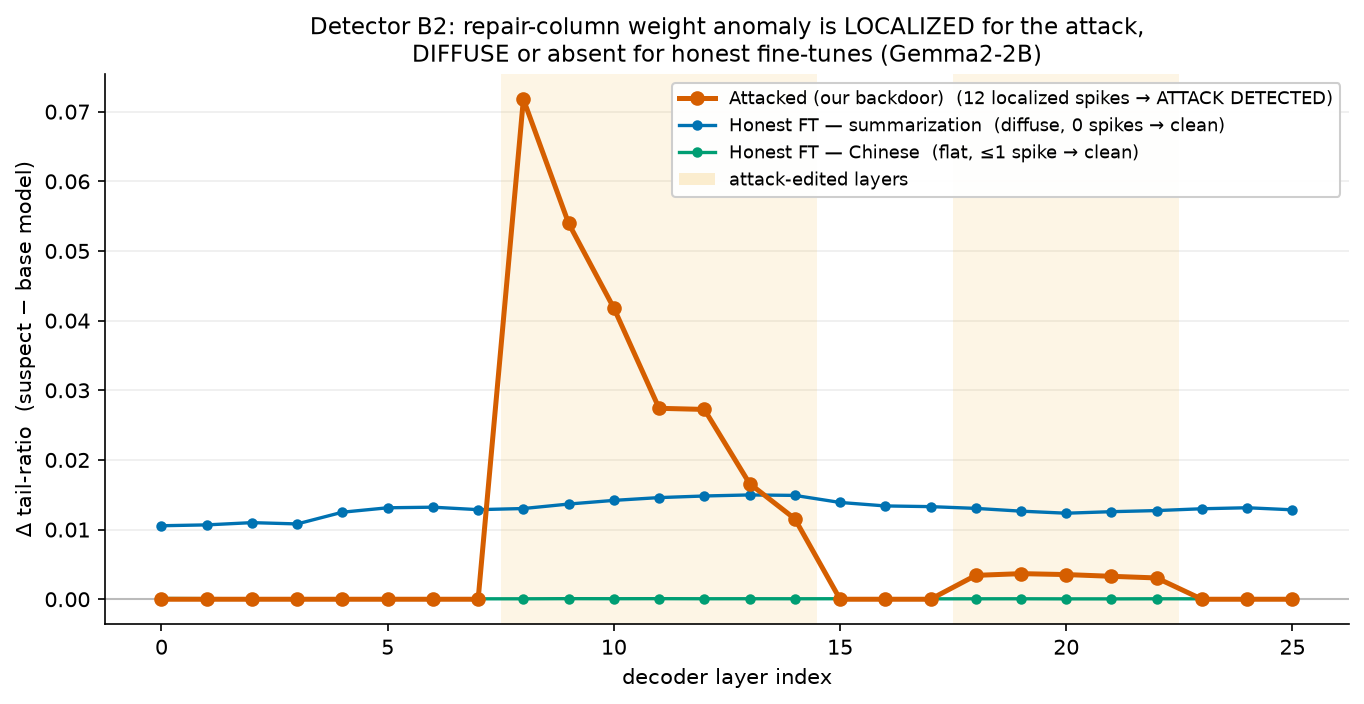
\includegraphics[width=0.9\linewidth]{defense_fig_gemma2.png}
\caption{Per-layer base-relative repair-column anomaly $\delta = \text{tail\_ratio}(\text{suspect}) -
\text{tail\_ratio}(\text{base})$ on Gemma2-2B. The attacked model ($\approx 0$ everywhere except sharp
bumps confined to the two edited bands, layers $8$--$14$ strong and $18$--$22$ weak) yields $12$
\emph{localized} outliers and is detected. An honest summarization fine-tune is \emph{uniformly}
elevated across all $26$ layers---the reason an absolute threshold false-positives---yet has $0$
localized spikes; an honest Chinese fine-tune is flat. The discriminative feature is
localization/sparsity, not magnitude.}
\label{fig:defense-gemma2}
\end{figure}

\begin{figure}[t]
\centering
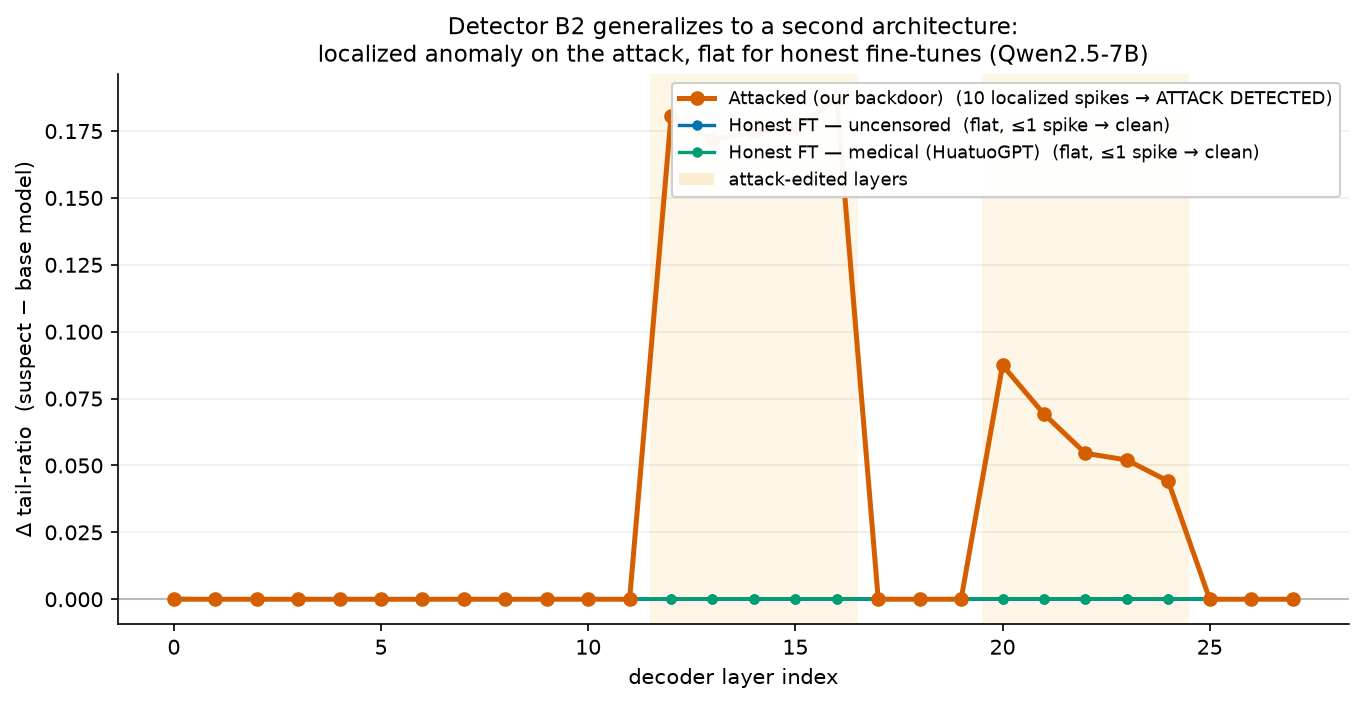
\includegraphics[width=0.9\linewidth]{defense_fig_qwen.png}
\caption{Detector~B2 on a second family, Qwen2.5-7B (attack edits layers $12$--$16$ and $20$--$24$).
All $10$ edited layers are flagged and none of the $8$ honest fine-tunes trip the $\geq\!2$-layer
rule; a repack of the base model scores $z=0$ exactly. Notably a deliberately \emph{uncensored}
fine-tune produces only a single stray edge-layer flag, so B2 detects the structural repair placement
rather than merely ``safety was weakened.''}
\label{fig:defense-qwen}
\end{figure}

\paragraph{Conclusions.}
The attack is stealthy against behavioral audits but \emph{not} against a base-diff weight audit when
the model is unmodified: Detector~A separates the edited layers from clean ones by a factor of
$10^{10}$. That defense, however, is defeated for free---an isotropic-noise ``fine-tune'' erases
Detector~A's signature at no cost to attack success (Table~\ref{tab:defense-noise})---so a base
difference is not a robust signal. The deployable detector is B2: a base-relative tail anomaly scored
for \emph{within-model localization}. It attains $100\%$ true-positive rate (every edited layer, both
architectures) with $0\%$ false positives across $18$ honest fine-tunes, and it survives the noise
camouflage that kills Detector~A, because isotropic perturbation inflates the MAD uniformly while the
localized repair spikes remain outliers. The defensible claim is therefore that the pruning-activated
backdoor resists naive weight audits under trivial camouflage, and that detecting it requires
\emph{localization-aware} weight-space auditing---which we provide a first, cross-architecture instance
of here.
